% !TEX TS-program = xelatex
% !TEX encoding = UTF-8 Unicode

\documentclass[AutoFakeBold]{LZUThesis2007}



\begin{document}
%=====%
%
%封皮页填写内容
%
%=====%

% 标题样式 使用 \title{{}}; 使用时必须保证至少两个外侧括号
%  如: 短标题 \title{{第一行}},  
% 	      长标题 \title{{第一行}{第二行}}
%             超长标题\tiitle{{第一行}{...}{第N行}}

\title{{《数据结构》课程的学习报告}}



% 标题样式 使用 \entitle{{}}; 使用时必须保证至少两个外侧括号
%  如: 短标题 \entitle{{First row}},  
% 	      长标题 \entitle{{First row}{ Second row}}
%             超长标题\entitle{{First row}{...}{ Next N row}}
% 注意:  英文标题多行时 需要在开头加个空格 防止摘要标题处英语单词粘连。
\entitle{{Study Report of Data Structres}}

\author{谭源}
\major{计算机类}
\advisor{蒙应杰}
\college{信息科学与工程学院}
\grade{2019级}



\maketitle

%======%
%诚信说明页
%授权说明书
%======%
\makestatement


\frontmatter



%中文摘要
\ZhAbstract{在计算机科学中,数据结构是计算机中存储、组织数据的方式。这学期蒙老师先由数据结构的定义开始讲起,依次讲解了算法、线性表、栈和队列、串、数组和广义表、树形结构、图结构、排序、数据检索这几部分内容

不要仅仅把它当做广告,这里面有很多latex的用法说明}{兰朵儿,i兰大易班,yuh}


%英文摘要
\EnAbstract{This essay explores the history of studies in analytical philosophy in China since the beginning of the last century, by dividing into three phases. It shows that, in these phases, analytic philosophy was always at a disadvantage in confronting serious challenges coming from both Chinese traditional philosophy and modern philosophical trends. The authors argue that Chinese philosophers have both done preliminary studies and offered their own analyses of various problems as well as some new applications of analytic philosophy especially in the latest period. Meanwhile, Chinese traditional philosophy was always trying to adjust its cultural mentality in the struggle with analytic philosophy, and accommodated in its own way the rationalistic spirit and scientific method represented in analytic philosophy.}
{analytical philosophy; Chinese philosophers; philosophical analysis;
dialogue in philosophy.
}

%生成目录
\tableofcontents


%文章主体
\mainmatter

\chapter{数据结构绪论}

其实我推荐绪论写在正文里!!作为第一章

    这里是绪论,也可以说是引言,在LZUThesis2020.clc里面改,引言写什么呢,先凑字数,

    是真的在打广告啊,嗯,做兰大毕业论文LaTex模板时,顺便介绍一下我写的软件:i兰大易班,兰大专属的app,可以看课表,充值校园卡(微信、支付宝都可以),查成绩(可以算绩点),还可以……,好多好多好多

    注意啊,段落在latex里面是要空一行的,不要简单一个回车

    \section{数据结构的基本概念及研究内容}

	数据元素:具有完整确定意义的描述现实的某一个客观实体的一个最小数据集。数据元素类似原子,可以再分,每一项被称作数据项

	数据对象:具有相同属性的数据元素的集合

	数据结构:给定数据对象及其上面定义的操作所共同构成的一个系统 一个信息处理模型

	主要研究的三个方面:
\begin{enumerate}
	\item 数据的逻辑结构
		\begin{itemize}
		\item  逻辑关系
	
					在自然形态下,数据元素之间的一种关系
	
		\item  逻辑结构
	
					数据之间所有关系的一个集合
				数学表示:B=(K,R),其中:
				K:数据上的有穷集合
				R:K上关系的有穷集合,其中每个关系r都是从K到K的关系
	
		\item  分类
	
			\begin{itemize}
				\item  线性
						
							一对一,单对单
		
				\item  非线性
				\begin{itemize}
					\item  树形结构
		
								唯一一个直接前驱,多个直接后继
		
					\item  图结构
				\end{itemize}
			\end{itemize}
		\end{itemize}

	\item 数据的存储结构
			\begin{itemize}
				\item  存储关系
	
							存储关系的数学内涵:须要建立数据对象(K)到存储区域(M)的映射关系(S):

							S:K→M

							即∀ k∈K,都有唯一的Z∈M ,使得S(K)=Z,Z为K结点所占存储空间的始单元。

	
				\item  存储结构
					\begin{itemize}
						\item  顺序结构
			
									按照连续地址空间的顺序依次的存放数据
			
						\item  链接结构

									存储密度相比顺序结构下降

						\item  索引结构
						\item  散列结构

									根据节点的值,通过一定的函数关系来确定数据元素的存储地址

					\end{itemize}
			\end{itemize}
	\item 数据的运算关系
				定义在逻辑结构上,在存储结构上实施,即:
				\begin{itemize}
					\item  抽象层面
						\begin{itemize}
							\item 逻辑关系
							\item 需求
						\end{itemize}
					\item  实现层面
						\begin{itemize}
							\item 存储关系
							\item 运算关系
						\end{itemize}
					\item  评价层面
				\end{itemize}
\end{enumerate}

三个层次五个要素

	\section{数据结构的选择与评价}
		评价标准:
			\begin{itemize}
				\item 时间需要量 时间效率
				\item 存储需要量 存储效率
			\end{itemize}

\chapter{算法}
	\section{算法的定义}
		\subsection{概述}

			算法是一个问题的具体解决方案

		\subsection{定义}

			算法解决某一个问题的指令的有限集合

			基本特征:
				\begin{itemize}
					\item 有穷性
					\item 确定性
					\item 可行性
					\item 输入
					\item 输出
				\end{itemize}

		\subsection{内涵及分类}
			内涵体现在过程上
				\begin{itemize}
					\item 一般过程
					\item 函数过程

						强调结果

				\end{itemize}

		\subsection{算法与程序的异同}
				\begin{itemize}
					\item 程序不是算法
					\item 程序不是算法 程序不一定满足有穷性
				\end{itemize}

	\section{算法的描述及设计原则}
		\subsection{算法描述方法}
			\begin{itemize}
				\item 计算机程序设计语言

					优点与缺陷:设计出=实现出

				\item 自然语言
					缺陷:雍长 二义性
				\item PDL
				\item 流程图
			\end{itemize}

		\subsection{算法基本标准}
			\begin{itemize}
				\item 正确性
				\item 易读性
				\item 健壮性
				\item 高效性
			\end{itemize}

	\section{算法分析概论及有效算法}
		\subsection{概念}

			一般不需要知道精确的时间消耗,需要知道时间消耗的增长率大体在什么范围。

			算法复杂性的阶:算法比较主要比较阶

			时间复杂性(时间渐进复杂性):利用某算法处理一个问题规模为n的输入所需要的时间,记为T(n)

			空间复杂性:利用某算法处理一个 问题规模为n的输入 所需要的存储空间,记为S(n)。

			阶:对一个正常数C,一个算法在时间Ο(n2)内能处理规模为n的输入,则称此算法的时间复杂度是Ο(n2),读作“n2 阶”,即该算法的时间复杂度与n2 是同阶的。

			\begin{figure}[H]
			    \centering
			    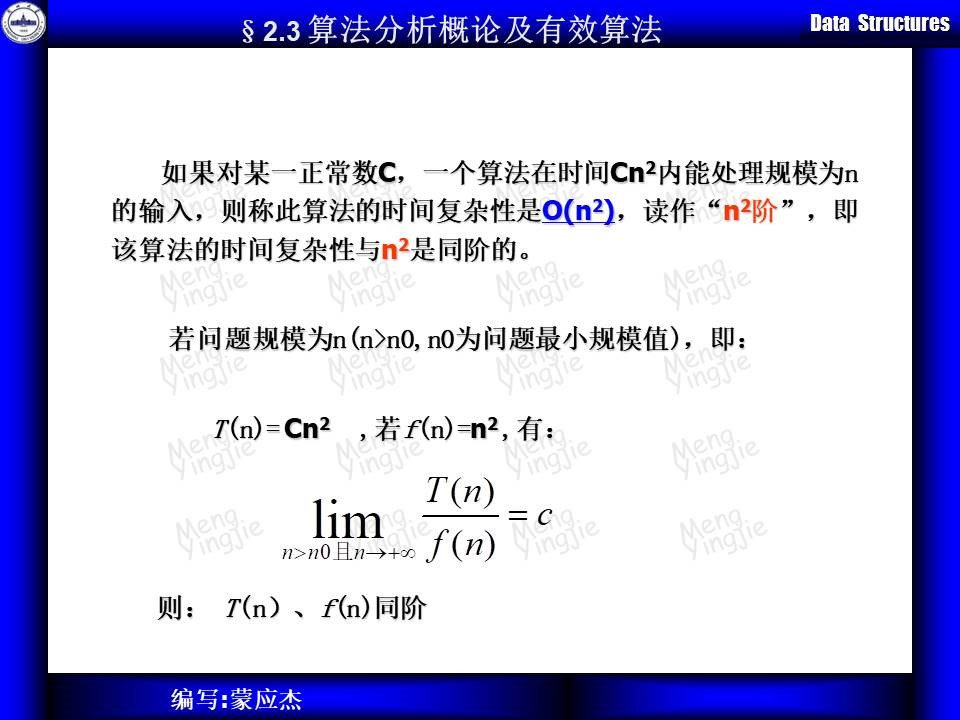
\includegraphics[width=0.7\textwidth]{figures/2.1.jpg}
			    \caption{启动图形化安装界面}
			    \label{fig_install_texlive}
			\end{figure}

			若一个算法时间复杂度为O(2n),称其需要指数时间;若是O(nk),称其为多项式时间。当n非常大时两个时间差异非常大。

			以多项式时间为界限的算法称为有效算法。如果一个问题不存在以多项式时间为界限的算法,称为难解的(难解性问题)

			\begin{figure}[H]
			    \centering
			    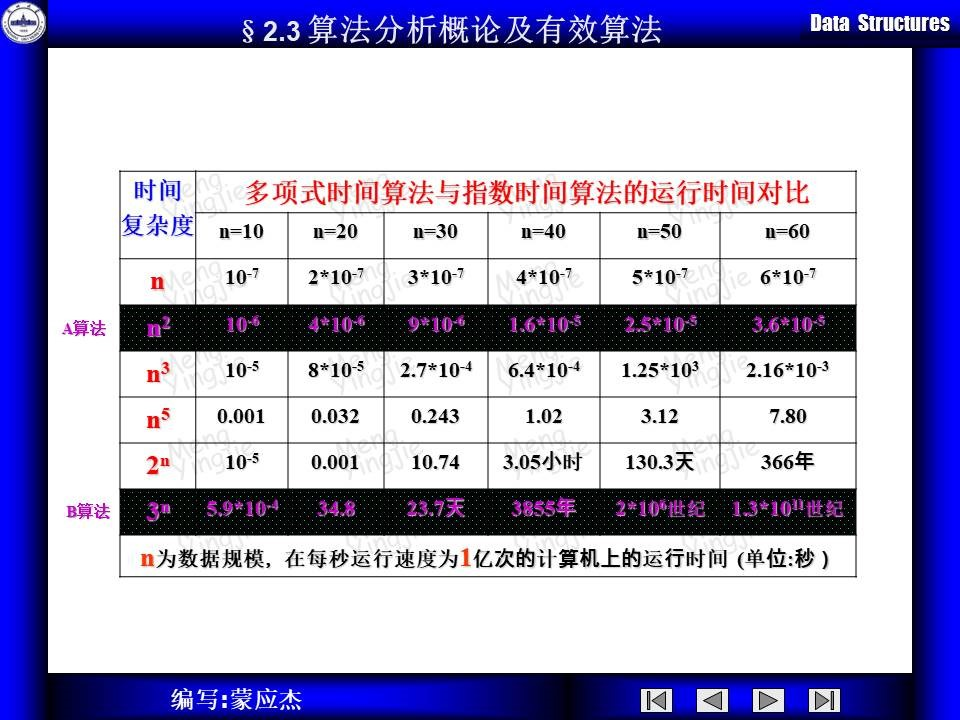
\includegraphics[width=0.7\textwidth]{figures/2.2.jpg}
			    \caption{启动图形化安装界面}
			    \label{fig_install_texlive}
			\end{figure}

			当n非常大时两个时间差异非常大。

			\begin{figure}[H]
			    \centering
			    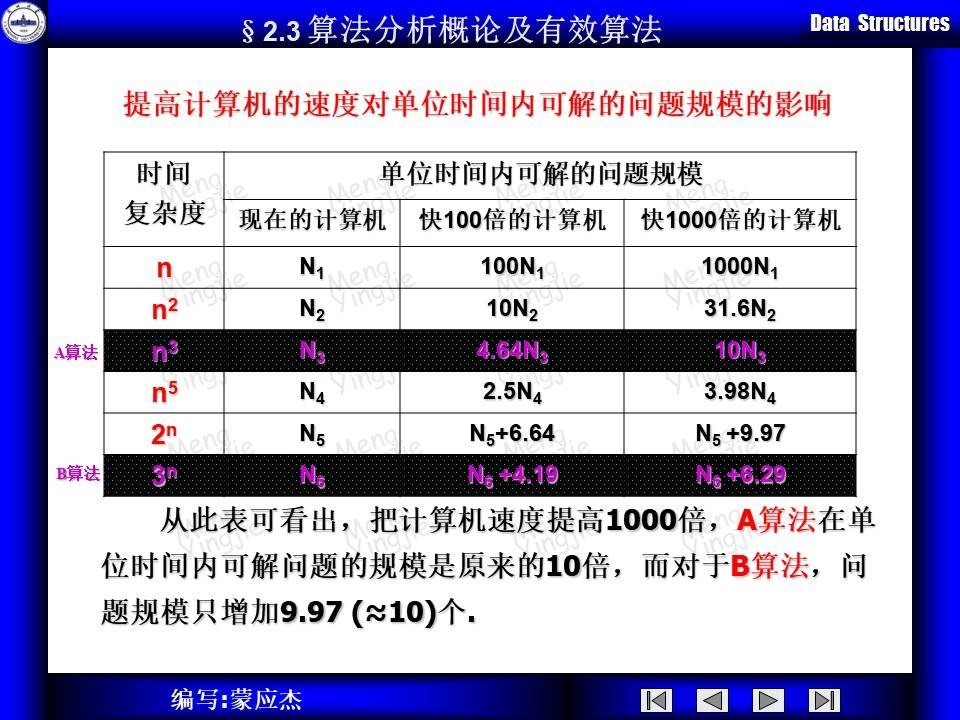
\includegraphics[width=0.7\textwidth]{figures/2.3.jpg}
			    \caption{启动图形化安装界面}
			    \label{fig_install_texlive}
			\end{figure}

			对于时间复杂度,会关注时间复杂度的ϱ最坏情况和时间复杂度的平均情况。

		\subsection{复杂性分析}

			不需要知道精确的数值,只需要知道他一个规模

			\begin{itemize}
				\item 时间复杂性的分析
					\begin{enumerate}
						\item 根据问题的特点合理选择一种或几种操作作为整个算法的“标准操作”(假设循环执行次数最多,循环就是标准操作)
						\item 确定每个算法在给定输入下总共执行了多少次标准操作,并根据次数推导求出时间函数
						\item 确定该函数的阶
					\end{enumerate}
				\item 空间复杂性的分析
					\begin{enumerate}
						\item 根据问题的特点合理选择一种或几种操作作为整个算法的“标准操作”(假设循环执行次数最多,循环就是标准操作)
						\item 确定每个算法在给定输入下总共执行了多少次标准操作,并根据次数推导求出时间函数
						\item 确定该函数的阶
					\end{enumerate}
				
					要求各个算法的存储结构一样的前提下,关注算法所需的附加存储空间复杂性

			\end{itemize}

	\section{算法设计方法概论}
		\subsection{概述}
			\begin{itemize}
				\item 用科学的方法进行算法设计
				\item 最常用方法:自顶向下 逐步求精

						顶层:问题的总和、抽象全貌

						底层:问题的具体化、展开、细节

						求精的方法:

					\begin{enumerate}
						\item 分而治之

								将问题划分为一些不相交的部分,依次解决

						\item 作出有限进展

								采用一个朝解的方向得到有限进展的方法,反复应用,逐渐逼近

						\item 情况分析

								对问题各种情况给予分析,选择适当方案。

					\end{enumerate}

				\item 健壮性
				\item 高效性
			\end{itemize}

		\subsection{算法设计的基本技术}
			以下内容不做要求
			\begin{itemize}
				\item 穷举法
				\item 分治法
				\item 回溯法
				\item 分支界限法
				\item 动态规划法
				\item 贪心法
			\end{itemize}

	\section{算法描述语言}
		\subsection{PDL概述}

			Program、Design、Language

			即伪码语言,主要用来书写软件设计的规约,是基于我们自然语言与具体的成设计语言之间的一种语言。这是一种保留计算机、程序设计、语言的基本框架和描述形式,并去掉一些特异性和直接性的要求,再结合自然语言所形成的一种用于描述算法处理的逻辑语言。

		\subsection{PDL的优势}
			\begin{itemize}
				\item 表达能力强,具有关键字的固定语法。提供了特定的结构化控制结构
				\item 引入了自然语言的一些习惯,结构比较清晰,简单易读
				\item 容易转化为任何一种程序设计语言代码(可由PDL生成程序代码)
			\end{itemize}

		\subsection{PDL书写及要求}
			\begin{enumerate}
				\item 算法的框架
					\begin{itemize}
						\item 一般过程的书写框架
\begin{lstlisting}
PROC 过程名(I/O参数);
BEGIN
	语句组
END;
\end{lstlisting}
						\item 函数过程的书写框架
\begin{lstlisting}
FUNC 函数名(I/O参数):类型名;
BEGIN
	语句组
END;
\end{lstlisting}
					\end{itemize}
				\item 词的定义及说明

						标识符:按照一定的规则形成的具有特定含义的一个词
						\begin{itemize}
							\item 过程名:调用前需定义
							\item 常量名、变量名:使用前需说明

									例如VAR i,j,k:integer

									常见的数据类型名写法及表示:
									\begin{itemize}
										\item 整数型:integer
										\item 实数型:real
										\item 布尔型:boolean
										\item 字符型(单字符):char
										\item 子介型(用于表达范围):下界..上界,例如40..90(表示40-90),'A'..'G'
										\item 枚举类型:{0,1,2,3}  元素次序不能变
										\item 构造类型
											\begin{itemize}
												\item 数组型:
\begin{lstlisting}
ARRAY[下标类型] OF 成分类型
\end{lstlisting}
												例如:
\begin{lstlisting}
A: ARRAY[1..20] OF integer
\end{lstlisting}
\begin{lstlisting}
B: ARRAY[1..20,-10..20] OF real	//(B是点集,二维数组)
\end{lstlisting}
												\item 记录型:
\begin{lstlisting}
RECORD
	域标识符1:类型1
	              …
	域标识符n:类型n
END
\end{lstlisting}
例如:
\begin{lstlisting}
A=RECORD
	Name:ARRAY[1…8] OF char;
	Sex:0..1
	Age:interger;
  END
\end{lstlisting}

											\end{itemize}
										\item 指针类型:
\begin{lstlisting}
↑ 类型名
\end{lstlisting}
例如:
\begin{lstlisting}
TYPE A=↑integer;		//指针类型
\end{lstlisting}
\begin{lstlisting}
VAR B:↑integer;			//指针变量
\end{lstlisting}

									\end{itemize}

						\end{itemize}
				\item 基本语序
					\begin{itemize}
						\item 赋值语句:
\begin{lstlisting}
变量名←表达式
\end{lstlisting}
						\item 流程图
						\item 条件语句
							\begin{itemize}
								\item 形式一
\begin{lstlisting}
if 条件 then 语句组
\end{lstlisting}
								\item 形式二
\begin{lstlisting}
if 条件 then 语句组1
	else 语句组2
\end{lstlisting}
							\end{itemize}
						\item 循环语句
							\begin{itemize}
								\item 当型(while)
\begin{lstlisting}
WHILE 条件 DO
	语句组;
\end{lstlisting}
								\item 直到型(repeat)
\begin{lstlisting}
REPEAT
	语句组;
UNTIL 条件
\end{lstlisting}
								\item 从到型(for-to)
									\begin{itemize}
										\item 默认步长为1:
\begin{lstlisting}
FOR 变量←初值 TO 终值 DO
	语句组;
\end{lstlisting}
										\item 自定义步长:
\begin{lstlisting}
FOR 变量←初值 TO 终值 STEP 步长值 DO
	语句组;
\end{lstlisting}
										\item 倒数:
\begin{lstlisting}
FOR 变量←初值 DOWNTO 终值 DO
	语句组;
\end{lstlisting}
									\end{itemize}

							\end{itemize}
						\item 输入语句:
\begin{lstlisting}
read(变量名表);
\end{lstlisting}
例:
\begin{lstlisting}
read(x,y,z);
\end{lstlisting}
						\item 输出语句
\begin{lstlisting}
write(变量名表);
\end{lstlisting}
					\end{itemize}
				\item 拓展语序
\begin{itemize}
	\item 情况语句
\begin{lstlisting}
CASE
	条件1:语句组1;
	条件2:语句组2;
	……
	条件n:语句组n;
	[ELSE 语句组n+1]
ENDCASE
\end{lstlisting}
	\item 一般过程调用语句:
\begin{lstlisting}
Call 过程名;
\end{lstlisting}
	\item 函数过程调用:通过在表达式中引用函数名完成,即被引用函数名出现在表达式中。
	\item 出错提示语句:
\begin{lstlisting}
error(错误信息);
\end{lstlisting}
	\item 终结语句
\begin{lstlisting}
Exit 	\\算法转向正常结束
\end{lstlisting}
\begin{lstlisting}
Return \\算法转向正常结束,携带值离开
\end{lstlisting}
\begin{lstlisting}
Abort 	\\中途废止(中止)
\end{lstlisting}
	\item 复合语句
\begin{lstlisting}
[ 	简单语句1;
	简单语句2;
	……
	简单语句n;	]
\end{lstlisting}
或用Begin End 代替括号

	\item 动态符号
\begin{itemize}
	\item 储存单元的引用:
\begin{lstlisting}
指针变量名↑
\end{lstlisting}
例:
\begin{lstlisting}
x↑
\end{lstlisting}
	\item 动态空间分配:
\begin{lstlisting}
New(P)
\end{lstlisting}
	\item 动态空间回收:
\begin{lstlisting}
Dispose(P)
\end{lstlisting}
	\item 空地址的表示:
\begin{lstlisting}
Nil
\end{lstlisting}
\end{itemize}
\end{itemize}
			\end{enumerate}

\chapter{线性表}
	\section{线性表及其运算}
		\subsection{线性表的定义}
		线性表的定义:一个线性表是n≥0个数据元素a1,a2,……,an的有限序列,序列中除第一及最后一个元素以外,每个元素有且只有一个直接前驱和直接后继。

		简称表,可表示为:A=(a1,a2,……,an)
\begin{lstlisting}
ai:datatype	//表示ai 项可以是任何类型
\end{lstlisting}

		\subsection{线性表的特征}
			\begin{itemize}
				\item 有限的。线性表的表长:线性表元素的个数。控标的长度定义为0
				\item 元素呈线性关系。元素的位置只取决于他们自己的逻辑顺序。
			\end{itemize}

		\subsection{线性表的运算}
			\begin{itemize}
				\item 确定线性表的长度n

				\item 存取线性表的第i个数据元素,检验或改变某个数据项的值
				\item 在第i-1个和第i个数据元素之间插入一个新的数据元素。约定插入的元素是第i个元素的直接前驱
				\item 删除第i个元素
				\item 将两个或两个以上的线性表合并成一个线性表
				\item 将一个线性表拆分成两个或两个以上的线性表
				\item 重新复制一个线性表
				\item 对线性表中的数据元素依据某一种规则进行重组
			\end{itemize}

	\section{线性表的储存表示}
\begin{itemize}
	\item 线性表的向量表示
		\begin{itemize}
			\item 存储方法
			顺序地分配存储单元,且每个数据元素占据相同大小的存储空间(顺序且等长)

			\item 数据访问
			TODO
			\item 向量存储结构特性
				\begin{itemize}
					\item 储存分配呈线性结构
					\item 属于随机存储结构(访问一个元素的代价与元素位置无关,即访问任何一个元素(找地址)的运算量一样,一维数组,通过下标变量来访问(数组构造的本质即算公式))

				\end{itemize}
			\item 向量存储结构的形式化表示
			可用一个一维数组表示,由于数组属于静态结构,其空间规模须事先定义(1..max),要有个计数器记录数组长度(空间规模)

			表述形式:
\begin{lstlisting}
TYPE SQLIST:ARRAY[1..max] OF datatype;							## 内容
VAR n:0..max;				                                 ## 计数器(记录数组长度)
\end{lstlisting}
\begin{lstlisting}
TYPE SQLIST= RECORD 
						data:ARRAY[1..max] OF datatype;
## 内容 n:0..max; ## 计数器(记录数组长度) 
       END;
\end{lstlisting}
			\item 插入
			\item 删除
			\item 小结
		\end{itemize}

	\item 线性表的链表表示
		\begin{itemize}
			\item 单链表表示
\begin{lstlisting}
TYPE pointer=↑node;
	node=RECORD 
			data: datatype;
			next: pointer;
		   END; 
	link=pointer;
\end{lstlisting}
			\item 带表头的单链表表示
			\item 带表头结点的循环单链表表示
			\item 带表头结点的双向循环链表表示
\begin{lstlisting}
TYPE pointer=↑node;
	node=RECORD 
			Left: pointer;
			data: datatype;
			
			right: pointer;
		   END;
	dblink=pointer;
\end{lstlisting}
		\end{itemize}
\begin{figure}[H]
    \centering
    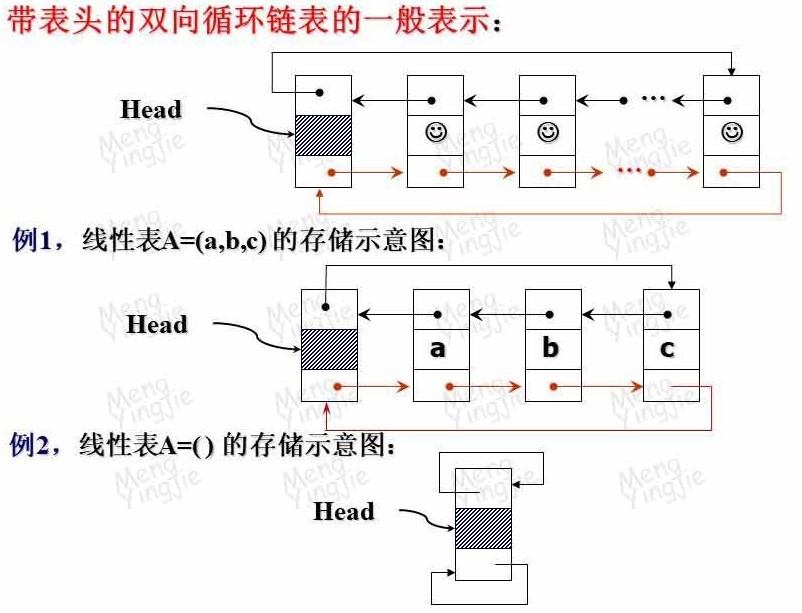
\includegraphics[width=0.7\textwidth]{3.1.jpg}
    \caption{启动图形化安装界面}
    \label{fig_install_texlive}
\end{figure}
\begin{figure}[H]
    \centering
    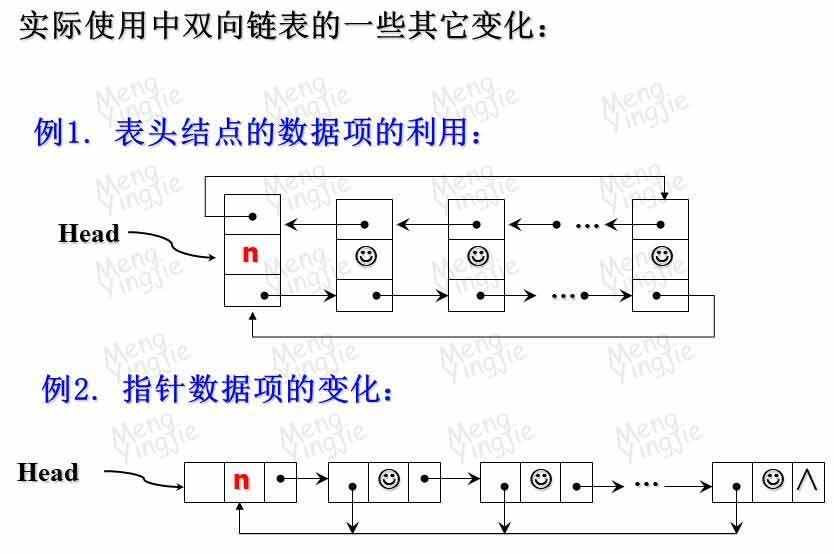
\includegraphics[width=0.7\textwidth]{3.2.jpg}
    \caption{启动图形化安装界面}
    \label{fig_install_texlive}
\end{figure}
	\item 线性表的应用
\end{itemize}


\chapter{栈和队列}
	\section{栈及其运算}
	栈是工具性数据结构
		\subsection{绪论}
		\subsection{栈的基本定义}
		栈是一个下限为常数,上限可变化的向量(或者反之)。有时称为堆栈或堆阵。

		后进先出表(LIFO)

		可变化一端称为栈顶,不变化的一端称为栈底

		\subsection{与线性表的关系}
			\begin{itemize}
				\item 相同点
					\begin{itemize}
						\item 逻辑关系都是线性关系
					\end{itemize}

				\item 不同点
					\begin{itemize}
						\item 线性表可以从任意位置增删,栈的增删只能从表尾进行
						\item 栈的运算是线性表的一个子集,且这个子集还需加以约束
					\end{itemize}

			\end{itemize}

		\subsection{栈的运算}
			\begin{itemize}
				\item 入栈,PUSH(S),完成往栈中加入元素的过程,即插入操作,也称为压栈
				\item 出栈,POP(S),完成从栈中取出元素的过程,即删除操作,也称为弹出
			\end{itemize}

		\subsection{栈的存储与运算的实现}
		\subsection{多栈共存问题}

	\section{栈的应用}

	\section{队列及其运算}
		\begin{itemize}
			\item 绪论
			分时和并行,主要处理对稀缺资源的争夺
			\item 队列的定义
			队列是一个下限和上限只能增加而不能减少(下限和上限的指针只能往一个方向移动)的向量(或者反之)

			先进先出表(FIFO)
			\item 队列与线性表
			\begin{itemize}
				\item 相同点
					\begin{itemize}
						\item 逻辑关系都是线性关系
					\end{itemize}

				\item 不同点
					\begin{itemize}
						\item 线性表可以从任意位置增删,队列的只能一端插入一端删除
						\item 队列的运算是线性表的一个子集,且这个子集还需加以约束
					\end{itemize}

			\end{itemize}
			\item 队列的运算
				\begin{itemize}
					\item 出队
					\item 入队
				\end{itemize}

			\item 队列的存储与运算的实现
		\end{itemize}

	\section{受限的栈及队列(了解)}
		\begin{itemize}
			\item 双端队列

			双端队列是一种所有的插入和删除都限制在表的两端进行的线性表
			\item 双栈

			双栈是一种加限制的双端队列,即从哪端进就只能从哪端出,就像是两个底部相连的栈
			\item 超队列

			超队列是一种删除受限制的双端队列,删除限制在一端,插入可以在两端
			\item 超栈

			超栈是一种插入受限制的双端队列,插入限制在一端,删除可以在两端
		\end{itemize}

\chapter{串}


\chapter{latex部分用法简介}

注意啊,看这个教程,template.pdf配合template.tex\textbf{一起看},才能学习latex怎么用的

网页跳转怎么用?图片插入怎么用?图片横着两个并排站呢?代码怎么插入?表格听说挺复杂?公式听说也挺难的

啥啥啥,你说你还不知道什么是LaTeX ,你去分不清XeLaTex、pdfLaTex,百度一下竟然还让我安装TexLive,这也就算了,甚至还有人说vscode?sublime text3?texstudio?Texmaker?我只是想写个论文排版方便一些,你要干嘛?

上面这些问题,后面都会一点点介绍

\section{用latex需要安装什么}
需要安装texlive,外加一个IDE

\subsection{texlive下载安装}
最近可能出了2020了,可以用兰大的镜像下载应该在用校园网时快一些,额,你还是用清华的镜像吧,我刚才找了一下,兰大镜像这会儿竟然挂了。。。

下载地址\footnote{这个地址会自动更新比如2020版出了以后你下载的就是2020了}: 点下面的字跳转浏览器下载了,方便吧

\begin{itemize}
	\item \href{https://mirrors.tuna.tsinghua.edu.cn/CTAN/systems/texlive/Images/texlive.iso}{TexLive2019 \quad Windows版}
	\item \href{http://tug.org/cgi-bin/mactex-download/MacTeX.pkg}{TexLive2019 \quad Mac版}
\end{itemize}

上面的文件直接双击安装一路next就行,但是texlive这是个啥?

用过python吧,texlive就相当于你下载的python安装包,但是你总不能在终端里写代码吧,一般用pycharm,这个就是IDE,所以你需要再安装一个IDE。


为什么没linux版?用的人不多,真心不想给。。。其实安装文件就是windows的那个版本

\subsubsection{linux系统图形界面安装texlive} % (fold)
\label{ssub:linux图形界面安装方式}

\begin{itemize}
	\item[1. ] 安装per组件: sudo apt-get install perl-tk
	\item[2. ] 加载该ISO文件:sudo mount -o loop texlive2019.iso /mnt (换掉文件路径即可)\footnote{注意:使用该命令会出现错误提示,mount: /dev/loop1 is write-protected, mounting read-only.不必管它}
	\item[3. ]启动图形化安装界面: cd /mnt \& sudo ./install-tl -gui
\end{itemize}

注意倒数第二项,改成 是,创建符号链接,下面那个图是网上随便找的,都差不多

\begin{figure}[H]
    \centering
    \includegraphics[width=0.7\textwidth]{figures/install_texlive.png}
    \caption{启动图形化安装界面}
    \label{fig_install_texlive}
\end{figure}



% subsubsection linux图形界面安装方式 (end)


\subsection{安装IDE} % (fold)
\label{sub:安装ide}

在这之前,请测试texlive是否安装成功!!!在命令行输入tex,显示类似如下结果,注意必须包含“TeX Live 2020”字样

\begin{lstlisting}[language=bash]
    This is TeX, Version 3.14159265 (TeX Live 2020) (preloaded format=tex)
    **
\end{lstlisting}


如果确实安装了,但是没有显示,请根据各自系统自行百度配环境变量,此处不再详细介绍


IDE这个就是写论文的地方,它会调用你刚才安装的texlive,具体用什么,各有所爱,我喜欢sublime text3,这个颜值是真的高,而且体积小,启动快,可以预览公式什么的,很多常用的代码可以自动提示补全,但是这个需要安装插件LaTexTools,pdf需要安装其他的东西进行正反向跳转\footnote{就是点tex文件某一行跳转到pdf对应的地方,点击pdf跳转到tex对应的那一行,mac上安装skim,windows安装sumatra},小白的话就算了吧,想折腾,百度一下吧


另外一个我比较喜欢的是vscode,也需要安装插件,很方便,和sublime text3差不多,但是用起来简单一些,也自己百度去吧

另外几个是\href{https://www.xm1math.net/texmaker}{Texmaker}、或者\href{http://texstudio.sourceforge.net/}{texstudio}\footnote{这个有可能需要番羽墙才能访问,什么意思,别问我,我不知道,啥都不知道},这两个你点名字就跳转官网了,这两个基本上是打开就可可以用,怎么用,自己百度吧,很多详细的图文教程


\begin{figure}[H]
	\centering
	\subfloat[sublime text3]{
        \includegraphics[width=0.4\textwidth]{figures/sublime.png}
    }\qquad
	\subfloat[vscode]{
        \includegraphics[width=0.4\textwidth]{figures/vscode.png}
    }\\
    \caption{我用的IDE}
    \label{fig_ide}
\end{figure}

这两个IDE真的是特别好用,不要再用TexMake或者TexStudio了,连个自动提示都麻烦,预览也没有,最主要的是太丑了,也不能换主题
% subsection 安装ide (end)



\section{常用的一些东西} % (fold)
\label{sec:常用的一些东西}

用到相关的直接到这里复制,然后修改就行

\subsection{国际三线表格} % (fold)
\label{sub:国际三线表格}

\begin{table}[H]
    \centering
    \caption{二硫化钼纳米管参数}
    \begin{tabular}{cccccc} % 控制表格的格式,可以是l,c,r
    \toprule
    参数& m & n & \tabincell{c}{太长了\\换行一下\\原子数}  & 内径 & 长度\\
    \midrule
    数值 & 15 & 15  & 2880 & 2.3014nm & 9.95nm \\
    \bottomrule
    \end{tabular}
    \label{tbl_mos2_nanotube}
\end{table}

这个注意,有多少列,后面就要有多少个c \footnote{否则会报错:Extra alignment tab has been changed to cr.有什么报错百度一下一般就找到了},这个c表示这一列居中(center),靠左的话:l,右:r;

那个label后面的名字自己取,但是不能有重复,是为了引用,比如这样,表格\ref{tbl_mos2_nanotube},方程、图片也是这样引用的,好处是,中间加一个表格导致这个表格的序号变了也没事,你不用再去修改其他地方的引用

\begin{lstlisting}[language = tex]
\begin{table}[H]
    \centering
    \caption{二硫化钼纳米管参数}
    \begin{tabular}{cccccc} % 控制表格的格式,可以是l,c,r
    \toprule
    参数& m & n & 原子数  & 内径 & 长度\\
    \midrule
    数值 & 15 & 15  & 2880 & 2.3014nm & 9.95nm \\
    \bottomrule
    \end{tabular}
    \label{tbl_mos2_nanotube_2}
\end{table}
\end{lstlisting}

\subsection{换页表格} % (fold)

我是真的没想到有的人表格居然这么长,竟然能有三页。。。。


\begin{longtable}{cccccc} % 控制表格的格式,可以是l,c,r
    \caption{二硫化钼纳米管参数}\label{tbl_mos2_nanotube}\\
    \toprule
    参数& m & n & 原子数 & 内径 & 长度\\
    \midrule
    数值 & 15 & 15  & 2880 & 2.3014nm & 9.95nm \\
    数值1 & 15 & 15  & 2880 & 2.3014nm & 9.95nm \\
    数值2 & 15 & 15  & 2880 & 2.3014nm & 9.95nm \\
    数值3 & 15 & 15  & 2880 & 2.3014nm & 9.95nm \\
    数值4 & 15 & 15  & 2880 & 2.3014nm & 9.95nm \\
    数值5 & 15 & 15  & 2880 & 2.3014nm & 9.95nm \\
    数值6 & 15 & 15  & 2880 & 2.3014nm & 9.95nm \\
    数值7 & 15 & 15  & 2880 & 2.3014nm & 9.95nm \\
    数值8 & 15 & 15  & 2880 & 2.3014nm & 9.95nm \\
    数值9 & 15 & 15  & 2880 & 2.3014nm & 9.95nm \\
    数值10 & 15 & 15  & 2880 & 2.3014nm & 9.95nm \\
    数值11 & 15 & 15  & 2880 & 2.3014nm & 9.95nm \\
    数值12 & 15 & 15  & 2880 & 2.3014nm & 9.95nm \\
    数值13 & 15 & 15  & 2880 & 2.3014nm & 9.95nm \\
    数值14 & 15 & 15  & 2880 & 2.3014nm & 9.95nm \\
    数值15 & 15 & 15  & 2880 & 2.3014nm & 9.95nm \\
    数值16 & 15 & 15  & 2880 & 2.3014nm & 9.95nm \\
    数值17 & 15 & 15  & 2880 & 2.3014nm & 9.95nm \\
    数值18 & 15 & 15  & 2880 & 2.3014nm & 9.95nm \\
    数值19 & 15 & 15  & 2880 & 2.3014nm & 9.95nm \\
    数值20 & 15 & 15  & 2880 & 2.3014nm & 9.95nm \\
    \bottomrule
\end{longtable}

    

% subsection 国际三线表格 (end)


\subsection{字体} % (fold)
\label{sub:字体}

\begin{table}[H]
    \centering
    \caption{字体}
    \begin{tabular}{ccccccc} % 控制表格的格式
    \toprule
    名称& 加粗 & 倾斜 & 宋体  & 仿宋 & 黑体 \\
    \midrule
    显示 & \textbf{兰朵儿} & \textit{兰朵儿}  & \songti{兰朵儿} & \fangsong{兰朵儿} & \heiti{兰朵儿}  \\
    显示 & \textbf{ldr} & \textit{ldr}  & \songti{ldr} & \fangsong{ldr} & \heiti{ldr}  \\
    \bottomrule
    \end{tabular}
    \label{tbl_font}
\end{table}
发现没,中文斜体没有效果的,你可以自定义,这个自己百度吧;而且加粗也windows系统上也是没有效果的,一般都改成了黑体(比如这个模板中成绩页等加粗的地方都是用的黑体),当然你也可以自定义。怎么做,百度吧



% subsection 常用的 (end)

\subsection{公式} % (fold)
\label{sub:公式}
所有的符号都要用美元符号包裹\$,需要用到某一个但是不知道,直接百度,基本上都有
\begin{table}[H]
    \centering
    \caption{公式}
    \begin{tabular}{cccccccccc} % 控制表格的格式
    \toprule
    名称& 分数 & 下角标 & 上角标  & 矢量 & 根号 & 希腊字母 & 点乘 & 叉乘 & 矢量\\
    \midrule
    显示 & $\frac{1}{2}$ & $O_2$  & $a^2$ & $\vec{AB}$ & $\sqrt[2]{3}$ & $\theta$ & $\cdot$ & $\times$& $\vec{a}$\\
   
    \bottomrule
    \end{tabular}
    \label{tbl_gs}
\end{table}

但是有时候我们只是正文中想用$MoS_2$,它竟然斜体,不想斜体,我写了个命令,这样用\eqrm{MoS_2},正的吧,常用的命令可以自定义

% subsection 公式 (end)

\subsection{左边大括号} % (fold)
\label{sub:左边大括号}

\begin{equation}
    \left\{
    \begin{array}{rcl}
        \vec{e_1} &= \frac{3a}{2} \vec{i} + \frac{\sqrt{3a}}{2} \vec{j} \\
        \vec{e_2} &= \frac{3a}{2} \vec{i} - \frac{\sqrt{3a}}{2} \vec{j}
    \end{array}
    \right.
    \label{e1e2}
\end{equation}

注意后面有个方程的编号,如果想取消,把上下的两个$equation$改成$equation*$

\begin{equation*}
    \left\{
    \begin{array}{rcl}
        \vec{e_1} &= \frac{3a}{2} \vec{i} + \frac{\sqrt{3a}}{2} \vec{j} \\
        \vec{e_2} &= \frac{3a}{2} \vec{i} - \frac{\sqrt{3a}}{2} \vec{j}
    \end{array}
    \right.
    \label{e1e2_2}
\end{equation*}

% subsection 左边大括号 (end)

\subsection{复杂公式} % (fold)
\label{sub:复杂公式}
不会输出的符号,请百度,啥都有

\begin{equation}
\hat{H}=\frac{\epsilon}{2}\hat{\sigma}_{z}-\frac{\Delta}{2}\hat{\sigma}_{x}+\sum_{k}\omega_{k}\hat{b}_{k}^{\dagger}\hat{b}_{k}+\sum_{k}\frac{g_{k}}{2}\hat{\sigma}_{z}(\hat{b}_{k}+\hat{b}_{k}^{\dagger})\label{eq:sbm}
\end{equation}

% subsection 复杂公式 (end)


\subsection{等号对齐站} % (fold)
\label{sub:等号对齐站}

主要是用这个aligned放在了方程的环境里,等号前面\&控制对齐,每一行后面双斜杠换行

\begin{equation}
    \begin{aligned}
        \vec{CH} & = m\cdot \vec{e_1} + n\cdot \vec{e_2} \\
        & = \frac{3(m+n)a}{2} \vec{i} + \frac{\sqrt{3}(m-n)a}{2} \vec{j} 
    \end{aligned}
    \label{ch}
\end{equation}

% subsection 等号对齐站 (end)

\subsection{矩阵乘法} % (fold)
\label{sub:矩阵乘法}

其实就是几个array组合

\begin{equation}
    \left[ 
    \begin{array}{c}
    x'\\
    y'\\
    \end{array}
    \right]=
    \left[ 
    \begin{array}{cc}
    cos \theta & sin \theta \\
    - sin \theta & cos \theta 
    \end{array}
    \right]
    \cdot
    \left[ 
    \begin{array}{c}
        x\\
        y\\
    \end{array}
    \right]
\end{equation}
% subsection 矩阵乘法 (end)


\subsection{图,并列排} % (fold)
\label{sub:图_并列排}

这一句代表这个图片宽度为一行文本宽度的$\frac{3}{10}$
\begin{lstlisting}[language = tex]
width=0.3\textwidth
\end{lstlisting}



\begin{figure}[H]
	\centering
	\subfloat[首页]{
        \includegraphics[width=0.3\textwidth]{figures/ldr1.jpg}
    }
	\subfloat[课表]{
        \includegraphics[width=0.3\textwidth]{figures/ldr2.jpg}
    }
	\subfloat[我的]{
        \includegraphics[width=0.3\textwidth]{figures/ldr4.jpg}
    }\\	
    \caption{i兰大易班截图}
    \label{fig_ldr}
\end{figure}

% subsection 图_并列排 (end)


\subsection{附页代码} % (fold)
\label{sub:附页代码}
可以在LZUThesis.clc里面修改代码格式

java代码
\begin{lstlisting}[language = java]
    System.out.print("i兰大易班")
    // 试一下中文注释
\end{lstlisting}


tex代码
\begin{lstlisting}[language = tex]
    width=0.3\textwidth
    % 注释
\end{lstlisting}

python代码
\begin{lstlisting}[language = python]
    print("i兰大易班")
    # 注释
\end{lstlisting}

matlab代码有专门的库,但是没必要高亮太多,而且中文适配有问题,直接按照下面这个就可以
\begin{lstlisting}[language = matlab]
    display("i兰大易班")
    % 注释
\end{lstlisting}

% subsection 附页代码 (end)

\subsection{参考文献} % (fold)
\label{sub:参考文献}

这个,百度学术、谷歌学术等网站都可以导出bibtex格式的参考文献(知网不行,网上有个人写了个转换器,但是windows用不了,就不放了,尽量用谷歌学术把那个文献找出来吧),直接放在bib/database.bib文件里、知网需要用其他东西转换,但是我建议用mendeley这个软件管理文献,然后可以导出bibtex格式的,甚至可以直接复制引用,很方便\cite{partl2016, tenne1992polyhedral, tussyadiah2015hotels}。

有些人希望多个参考文献同时引用时用[1-3]而不是[1,2,3],所以我加了个包cite。(2020-5-18)

具体怎么用可以百度,我这里告诉你什么可以用,但是具体的,建议百度,更靠谱一些。


有参考文献时,编译要经过4步,直接XeLaTeX --> BibTeX --> XeLaTeX --> XeLaTeX,不然很多问题,我用的sublime text3,配合插件LatexTool,直接快快捷键ctrl - B,就可以自动完成4步了,很方便

% subsection 参考文献 (end)

% section 图标等常用的教程 (end)




%论文后部
\backmatter


%=======%
%引入参考文献文件
%=======%
\bibdatabase{bib/database}%bib文件名称 仅修改bib/ 后部分
\printbib
% \nocite{*} %显示数据库中有的,但是正文没有引用的文献



\Appendix


这里是附录页,附上你的程序或必要的相关知识

{\bfseries 编译方式:} XeLaTeX -->BibTeX --> XeLaTeX-->XeLaTeX


\Thanks

这里是致谢页,你可以在这里致谢你的舍友,老师,朋友,或者我。


%=====%
%论文(设计)成绩:注意2007的模板要求,成绩页在最后,2020要求成绩页在摘要前面
%=====%

% 下面这些注释掉可以去掉成绩、评语什么的
\supervisorcomment{导师评价你人很好}

\recommendedgrade{80}

\supervisorsignature{
    \raisebox{-10pt}{
        \includegraphics[width=60pt]{signature.pdf}
    }
}

\committeecomment{优秀}

\finalgrade{100}
% 上面这些注释掉可以去掉成绩、评语什么的

\Grade %这一句才是成绩页,上面是填写


\end{document}